\setchapterstyle{lines}
\chapter{Additional Figures}
\label{ch:additional-figures}

\section{Event Selection}

\subsection{Seasonal Stability of Variables (KS Tests)}
\label{sec:ks-test-appendix}

\reffig{data_stability_2D_control_KS} shows heat maps of the p-value calculated between each pair of seasons used in the data sample underlying this work. The null hypothesis of the test is that the samples of each season are drawn from the same distribution. The top row shows the results for the analysis variables energy, zenith angle and PID, while the bottom row shows the results for three selected control variables. 

\begin{figure*}
  \begin{center}      
      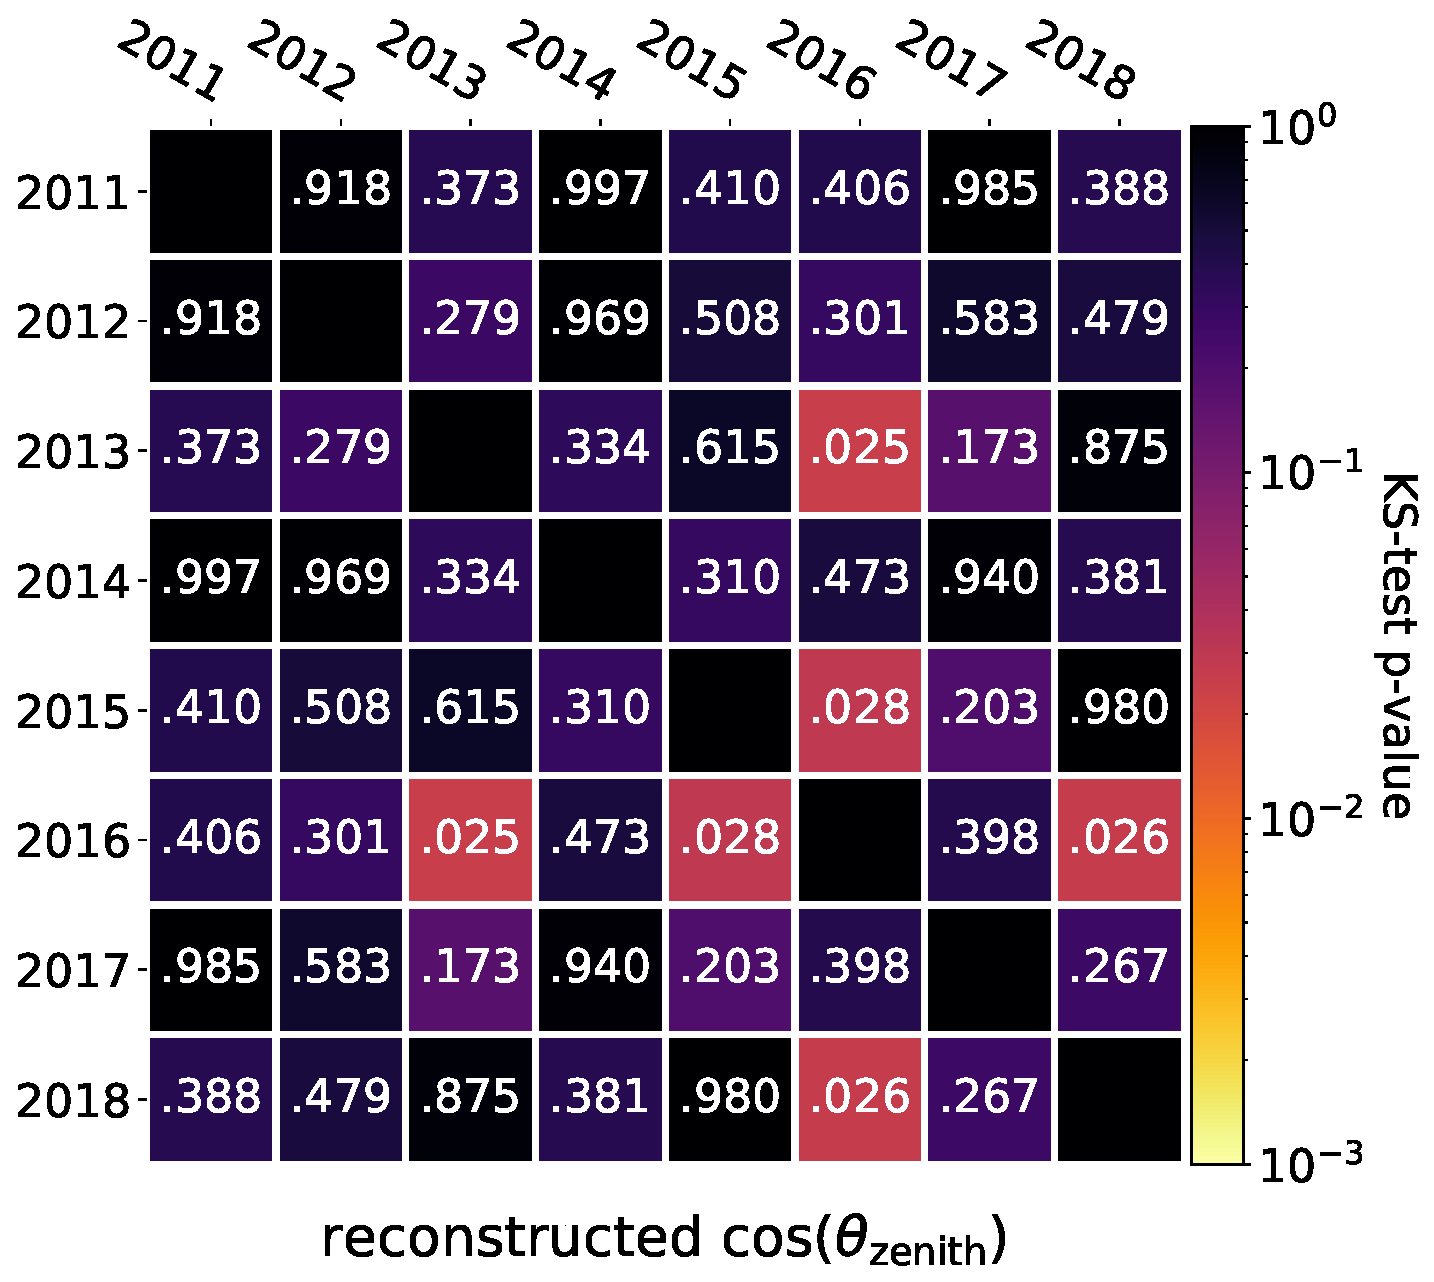
\includegraphics[width=0.3 \linewidth]{figures/icecube/selection/data_stability/KS_tests/ks_map_L6_SANTA_sel_Particle.coszen_final_level_binning.pdf} 
      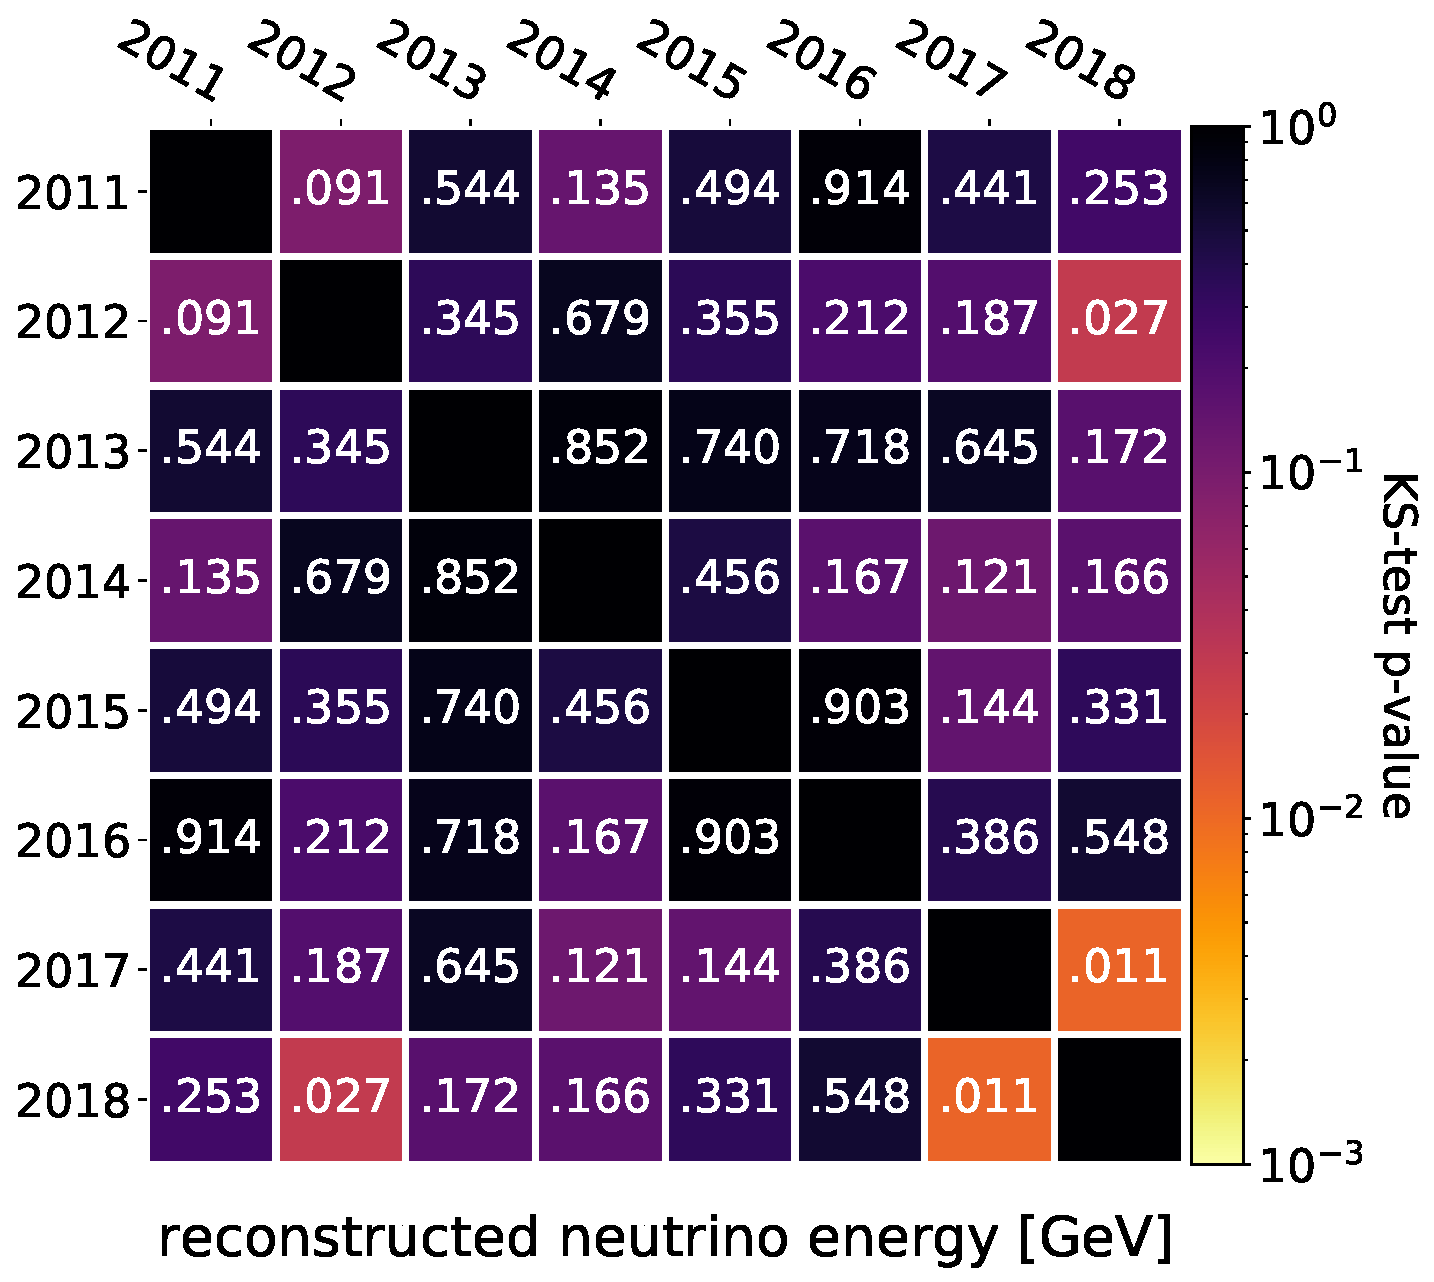
\includegraphics[width=0.3\linewidth]{figures/icecube/selection/data_stability/KS_tests/ks_map_L7_SANTA_sel_LEERAFit_result_dict.NeutrinoEnergy_final_level_binning.pdf}
      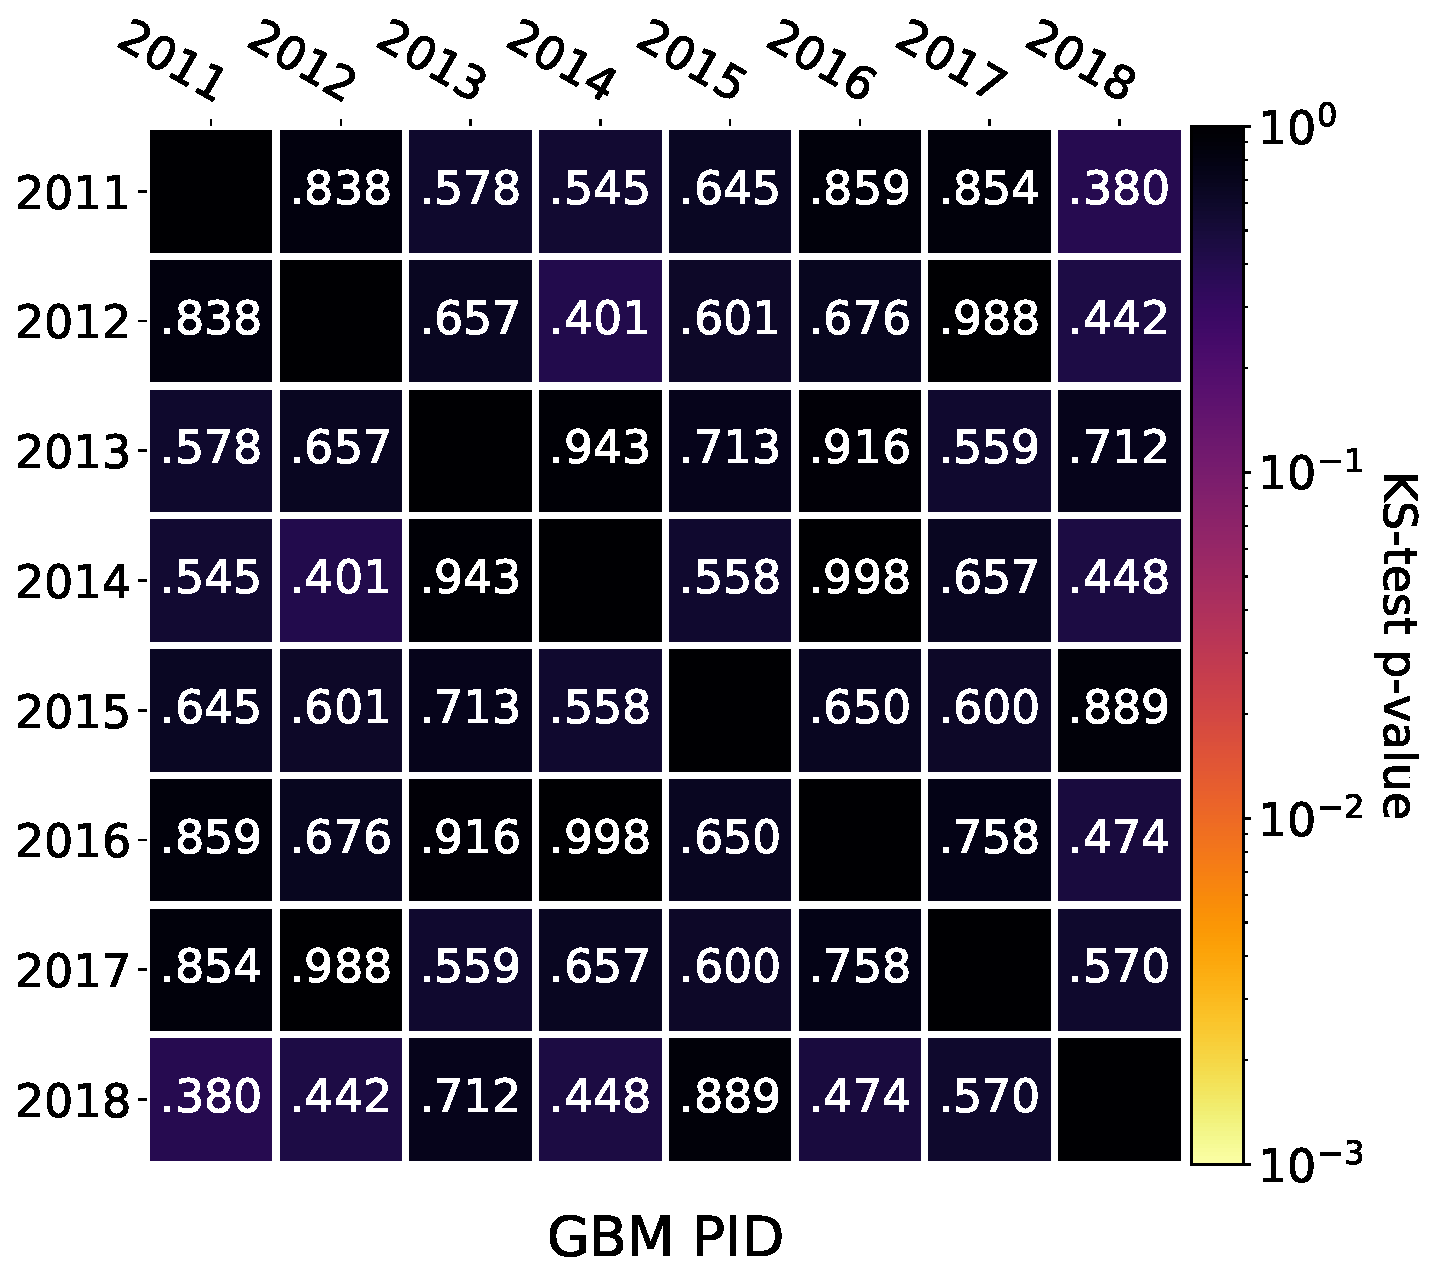
\includegraphics[width=0.3 \linewidth]{figures/icecube/selection/data_stability/KS_tests/ks_map_GBM_PID_final_level_binning.pdf}\\
  \end{center}
  \begin{center}      
      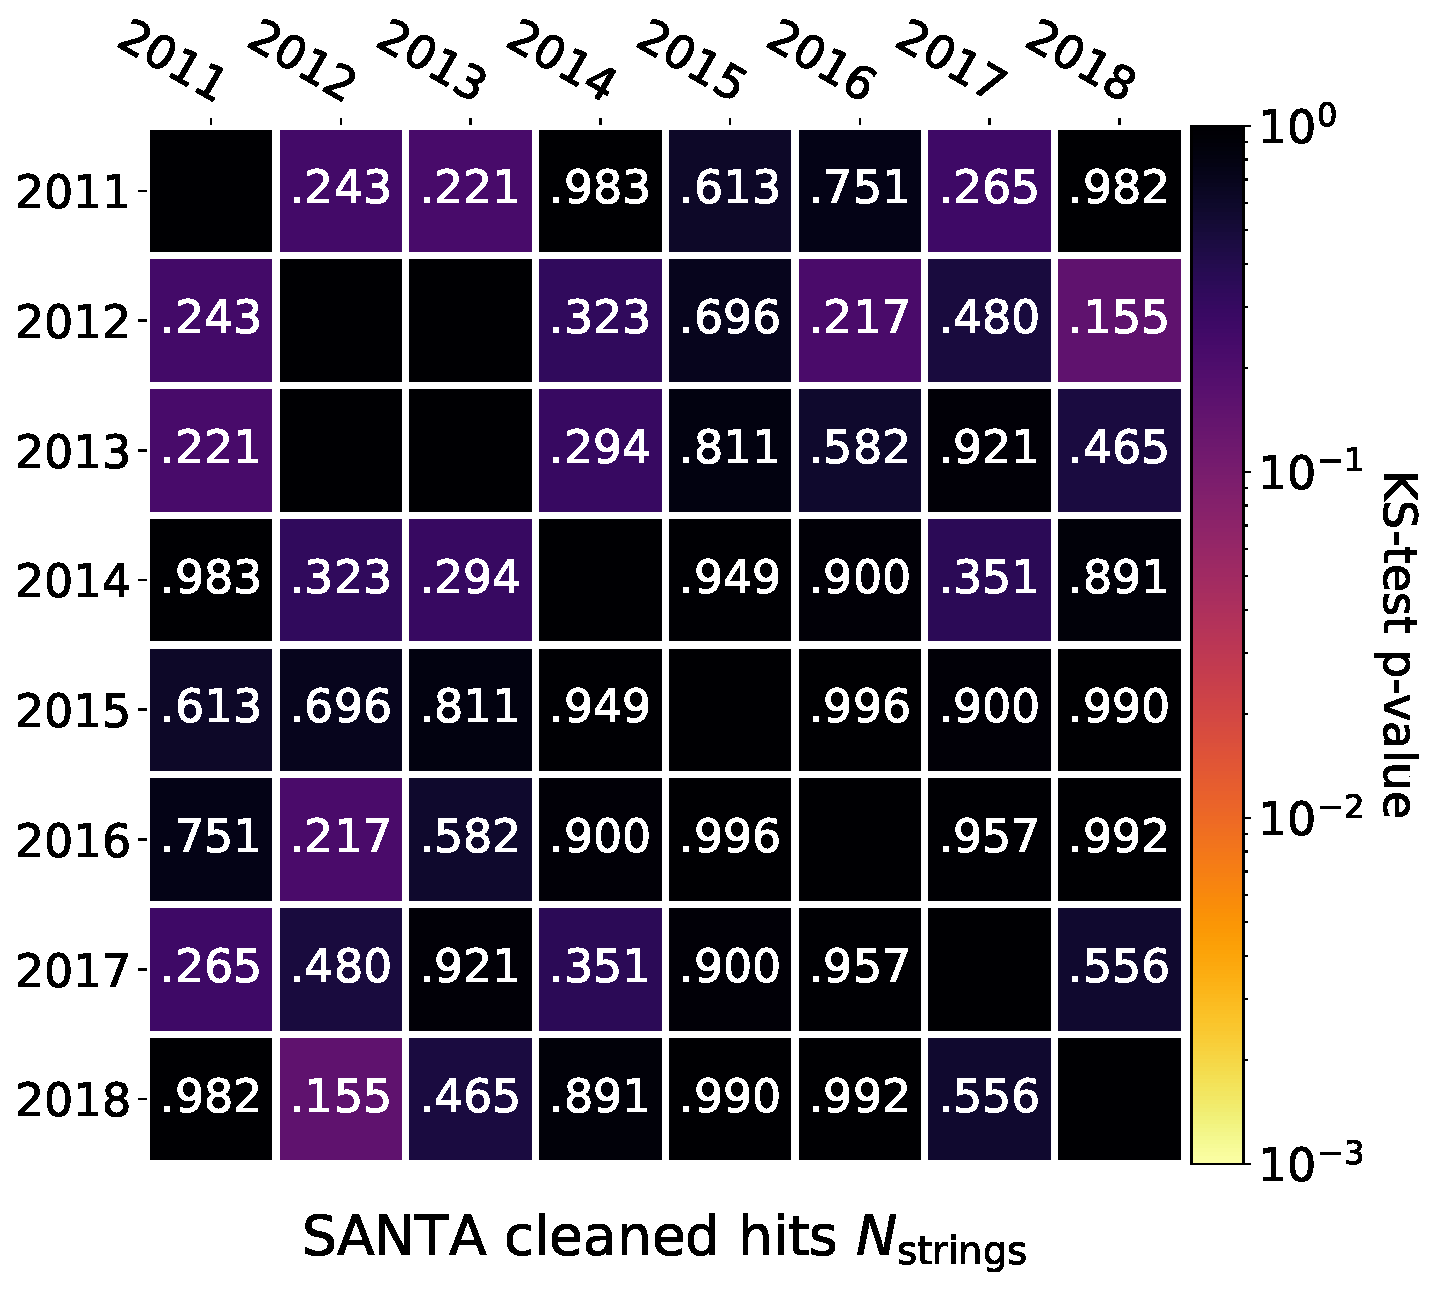
\includegraphics[width=0.3\linewidth]{figures/icecube/selection/data_stability/KS_tests/ks_map_L5_SANTA_DirectPulsesHitMultiplicity.n_hit_strings_final_level_binning.pdf}
      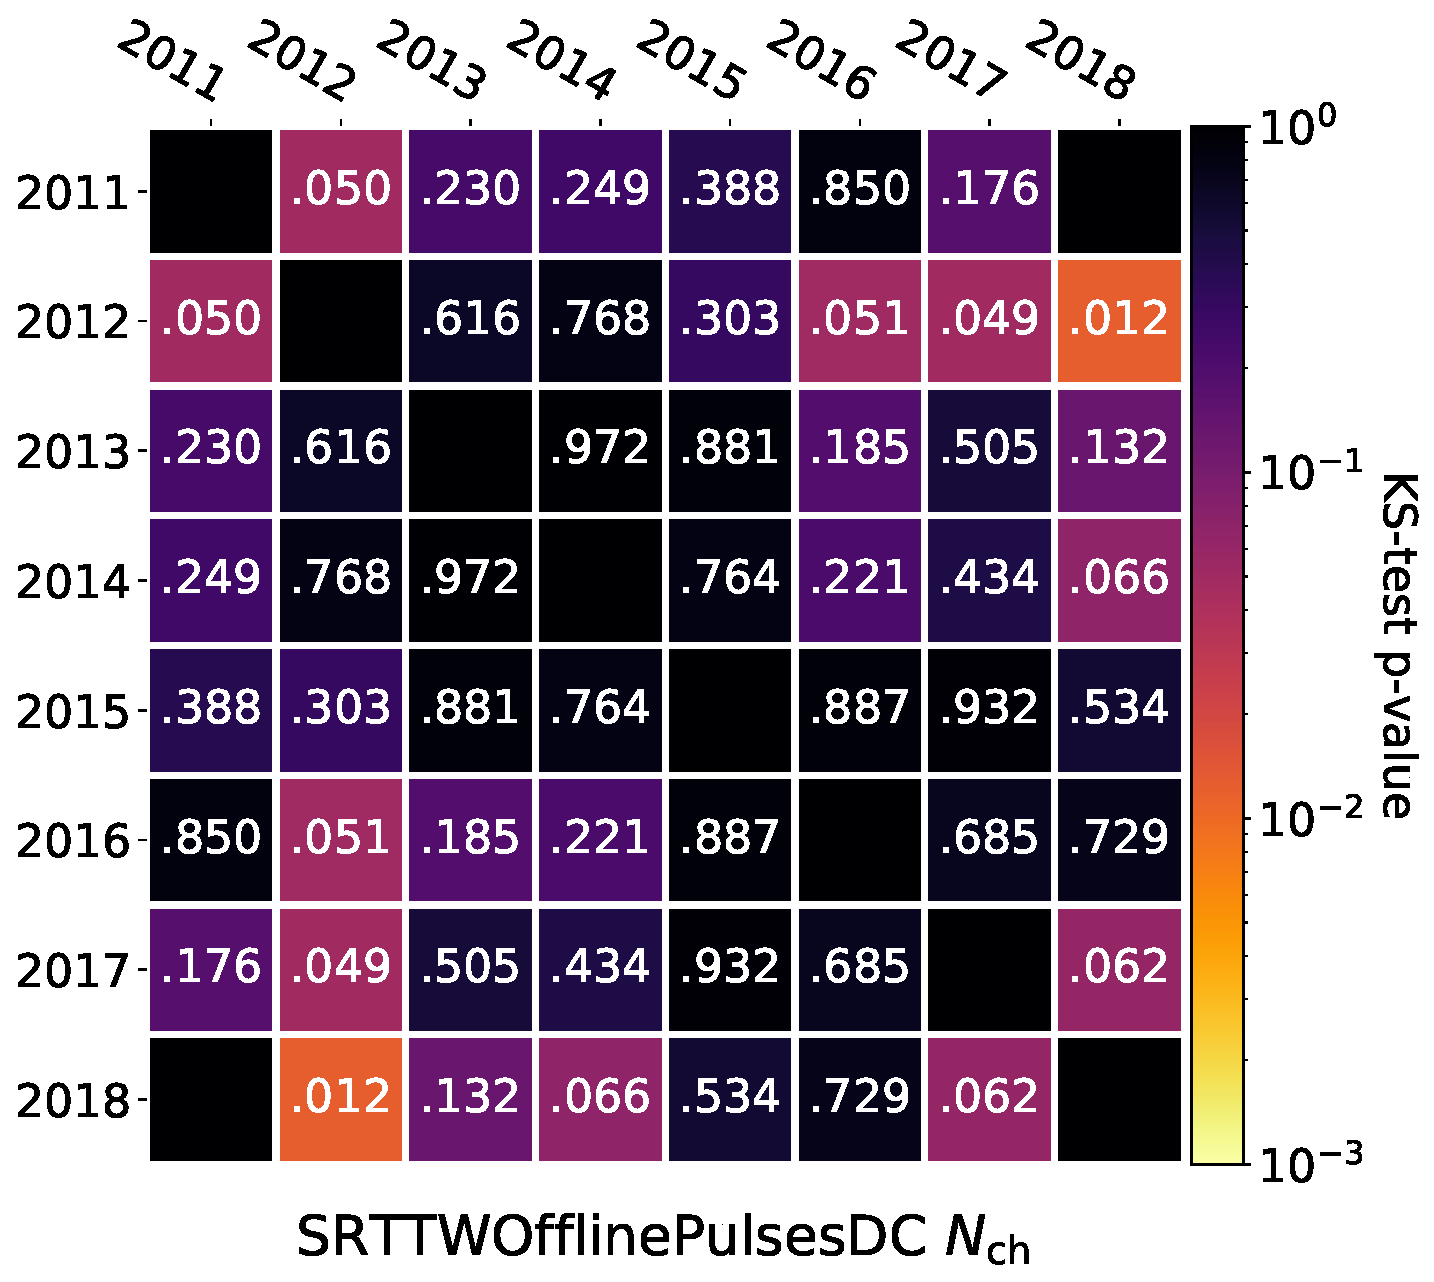
\includegraphics[width=0.3 \linewidth]{figures/icecube/selection/data_stability/KS_tests/ks_map_SRTTWOfflinePulsesDCHitMultiplicity.n_hit_doms_final_level_binning.pdf}
      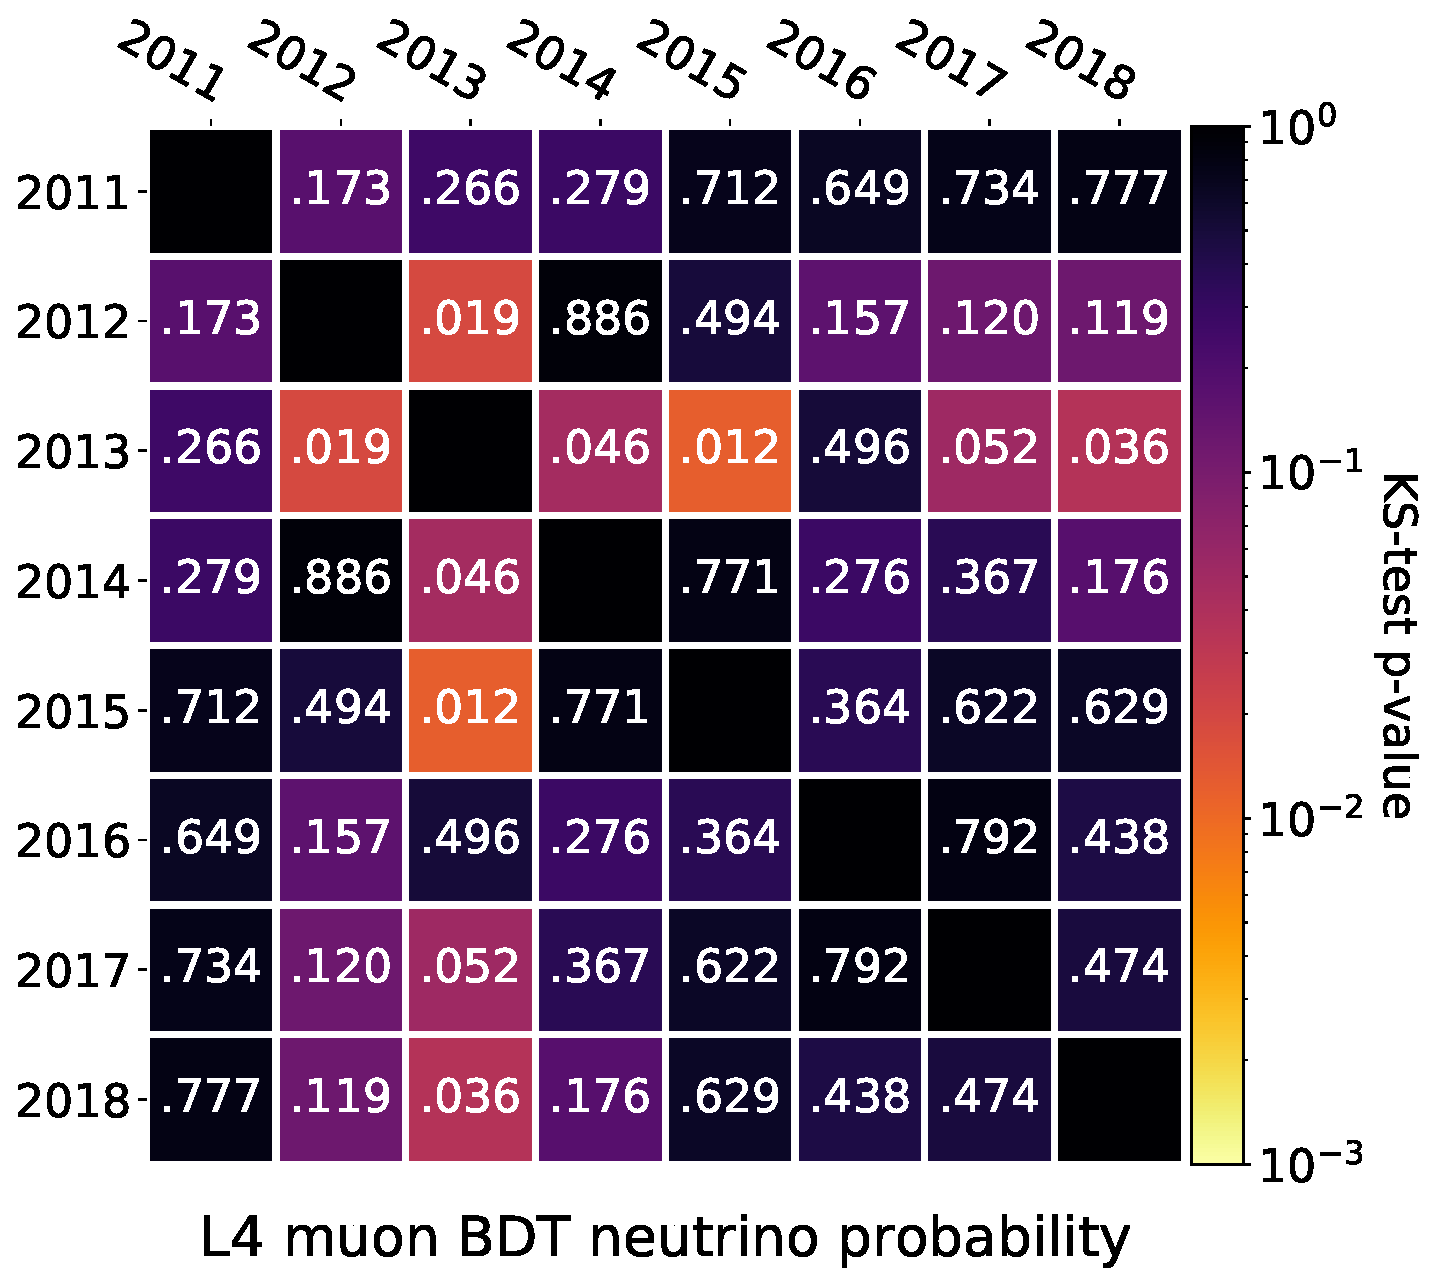
\includegraphics[width=0.3 \linewidth]{figures/icecube/selection/data_stability/KS_tests/ks_map_L4_MuonClassifier_Data_ProbNu_final_level_binning.pdf}
  \end{center}
  \caption{Kolmogorov-Smirnov p-values calculated between each season of data for reconstructed quantities used in the fit (top) and control variables (bottom)}
  \label{fig:data_stability_2D_control_KS}
\end{figure*}


\subsection{PID Variables}
\label{sec:apx-pidvars}
Histograms showing the distributions of variables used for event signature classification (see section~\ref{sec:pid}).

\begin{figure*}
    \centering
    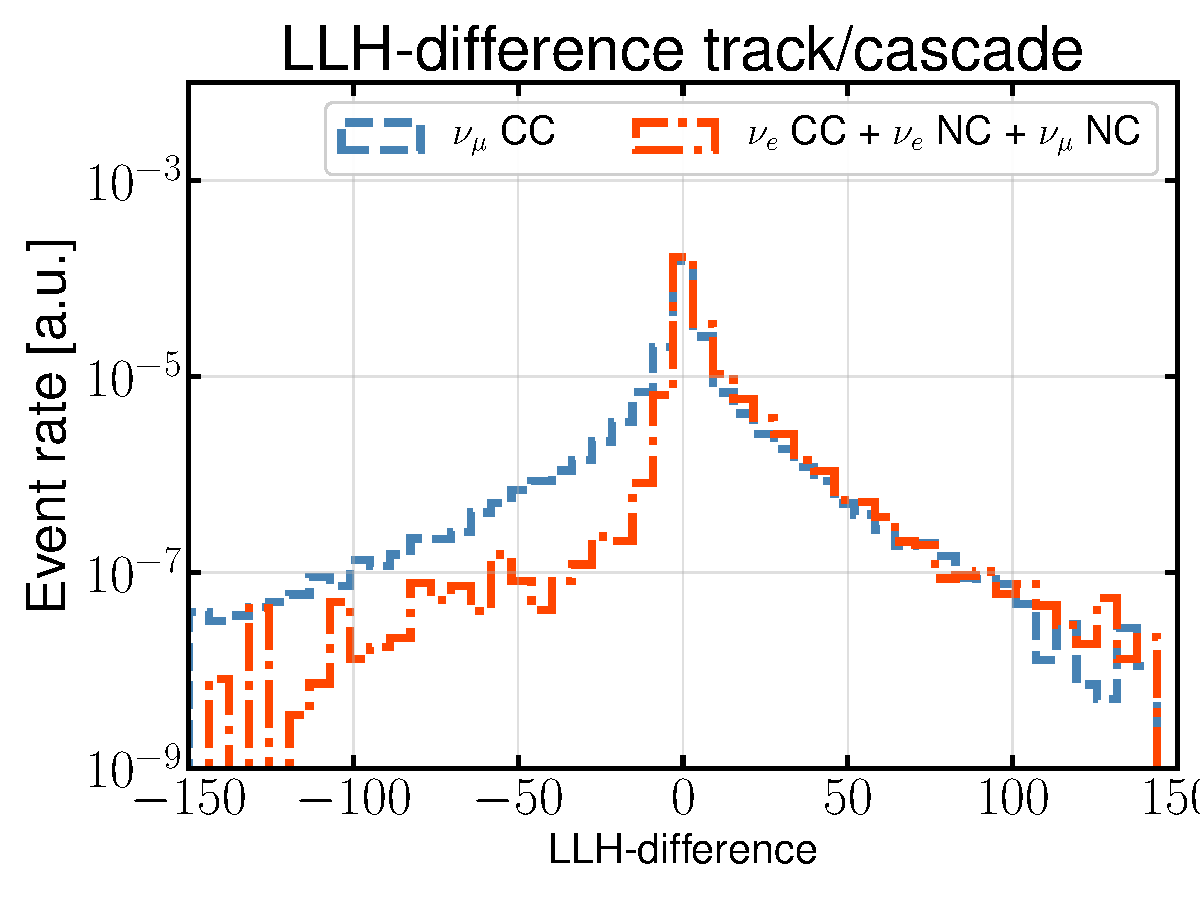
\includegraphics[width=0.49\linewidth]{figures/icecube/classification/variables/leera.pdf}
    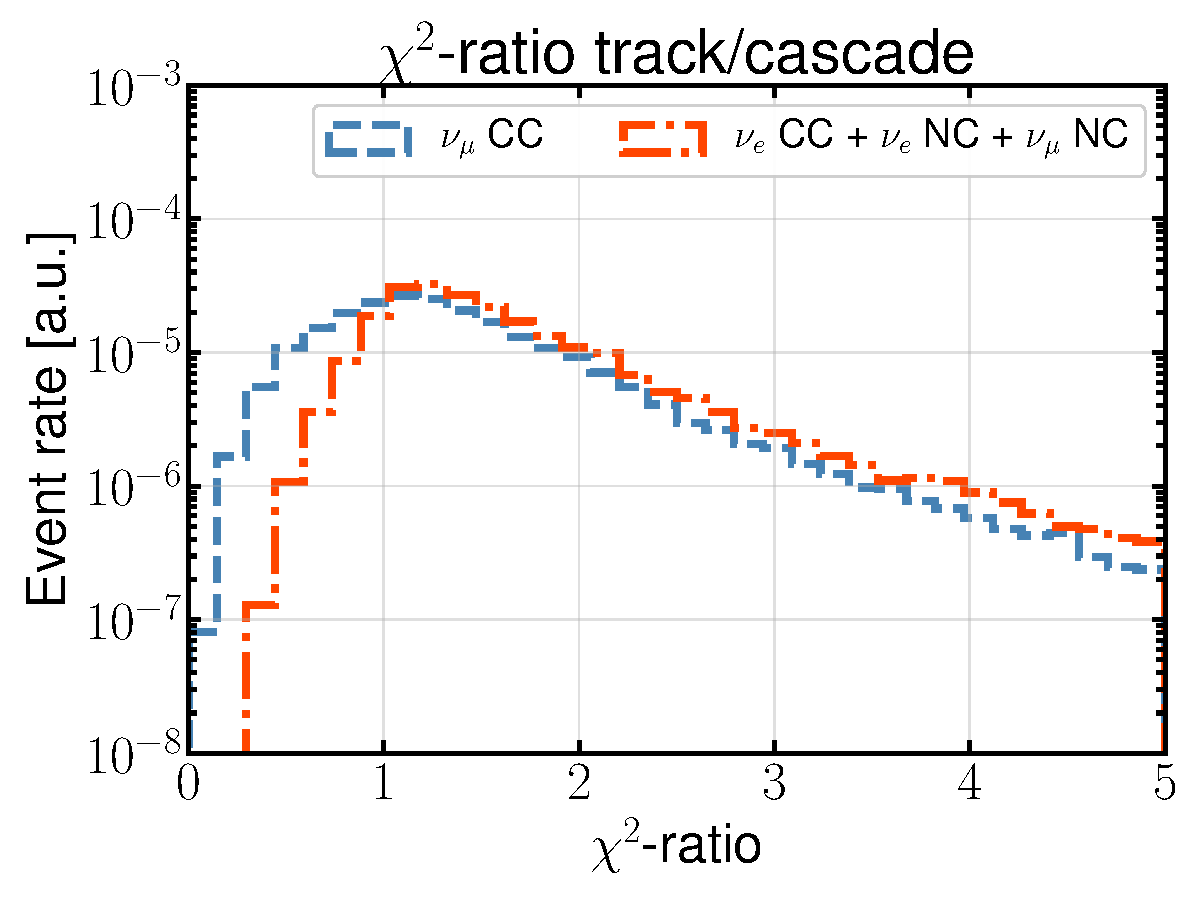
\includegraphics[width=0.49\linewidth]{figures/icecube/classification/variables/santa.pdf}
    \caption{Histograms of the likelihood score from the energy reconstruction (left) and the goodness-of-fit ratio of the zenith reconstruction (right) in simulation.}
    \label{fig:apx-pidvars-santa-leera}
\end{figure*}

\begin{figure*}
    \centering
    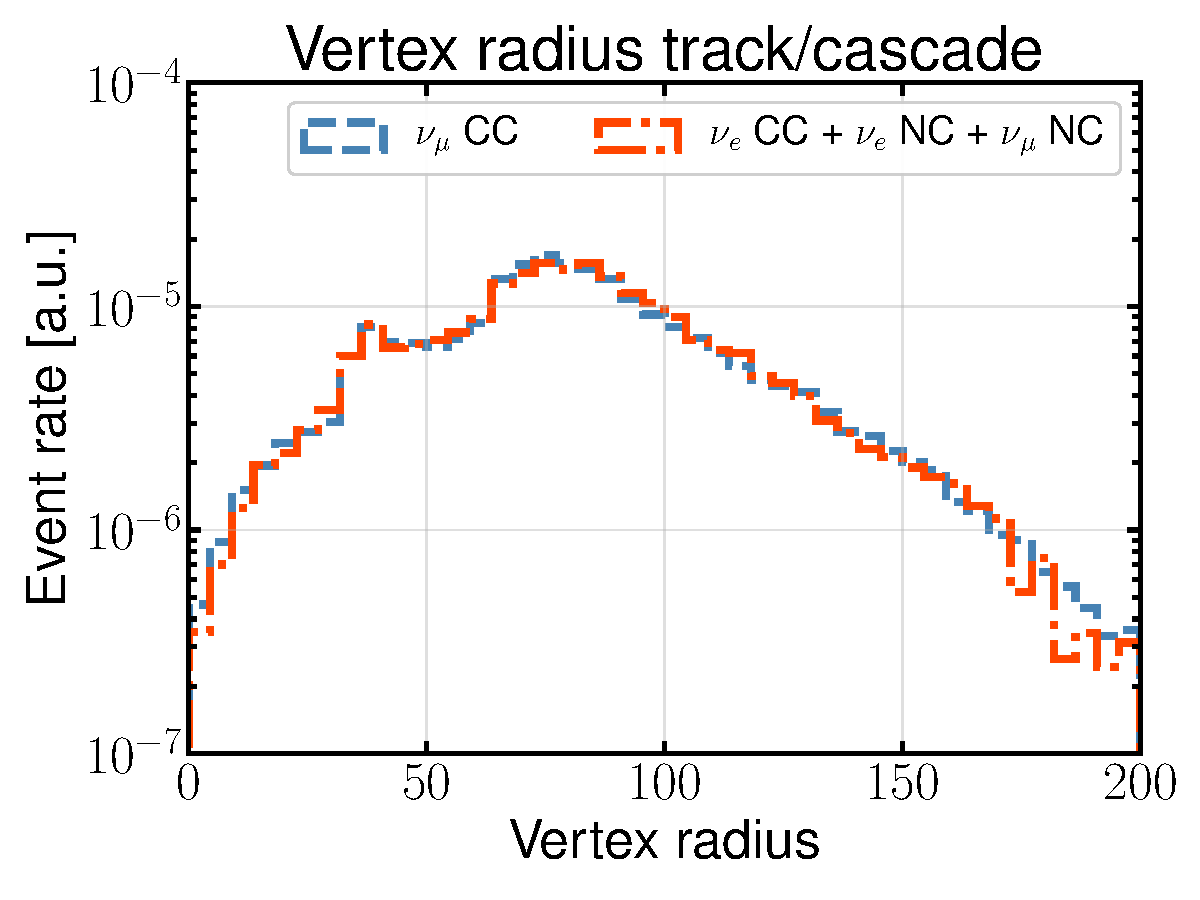
\includegraphics[width=0.49\linewidth]{figures/icecube/classification/variables/rho36_start.pdf}
    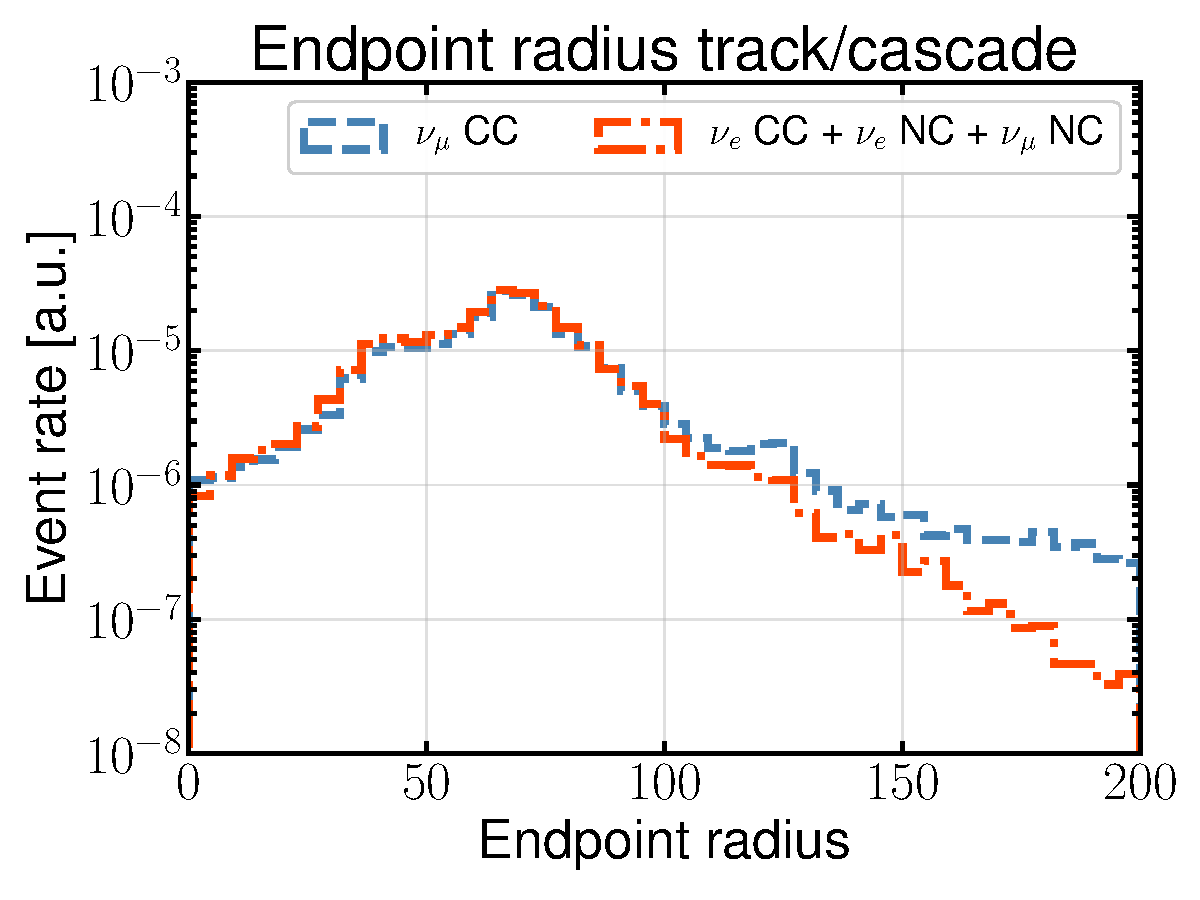
\includegraphics[width=0.49\linewidth]{figures/icecube/classification/variables/rho36_end.pdf}
    \caption{Histograms of the radius with respect to string 36 of the vertex (left) and the endpoint of the reconstructed track (right) in simulation.}
    \label{fig:apx-pidvars-rho36}
\end{figure*}

\begin{figure*}
    \centering
    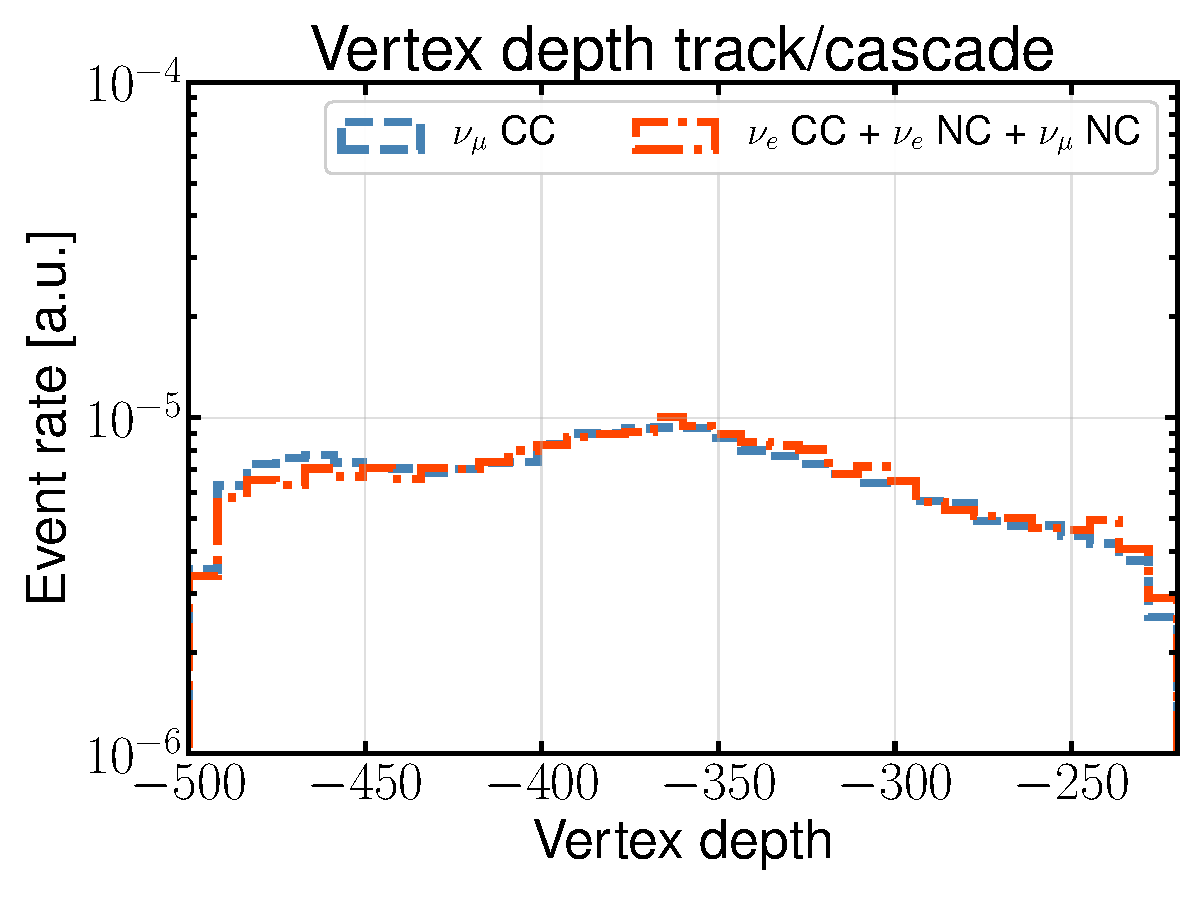
\includegraphics[width=0.49\linewidth]{figures/icecube/classification/variables/z_start.pdf}
    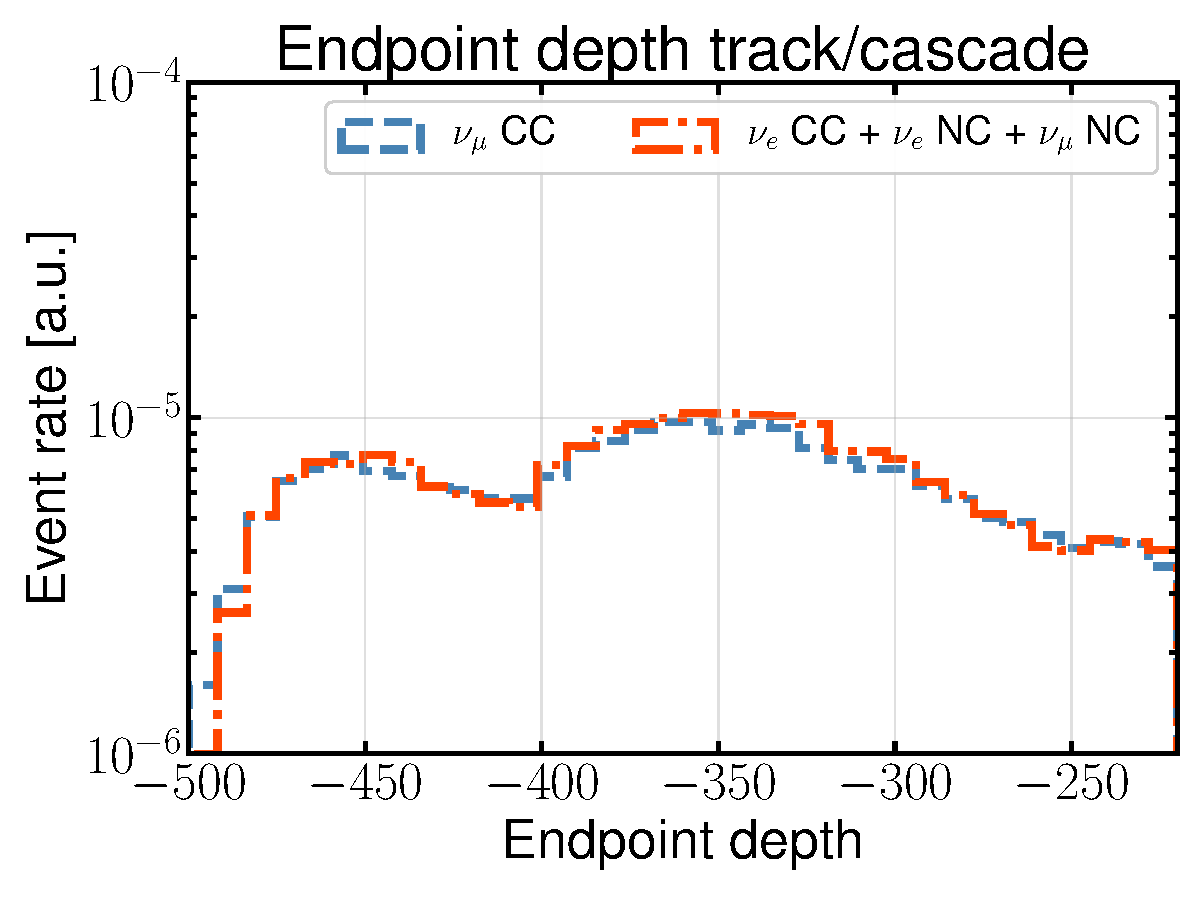
\includegraphics[width=0.49\linewidth]{figures/icecube/classification/variables/z_end.pdf}
    \caption{Histograms of the z-coordinate of the vertex (left) and the endpoint of the reconstructed track (right) in simulation.}
    \label{fig:apx-pidvars-z}
\end{figure*}

\begin{figure*}
    \centering
    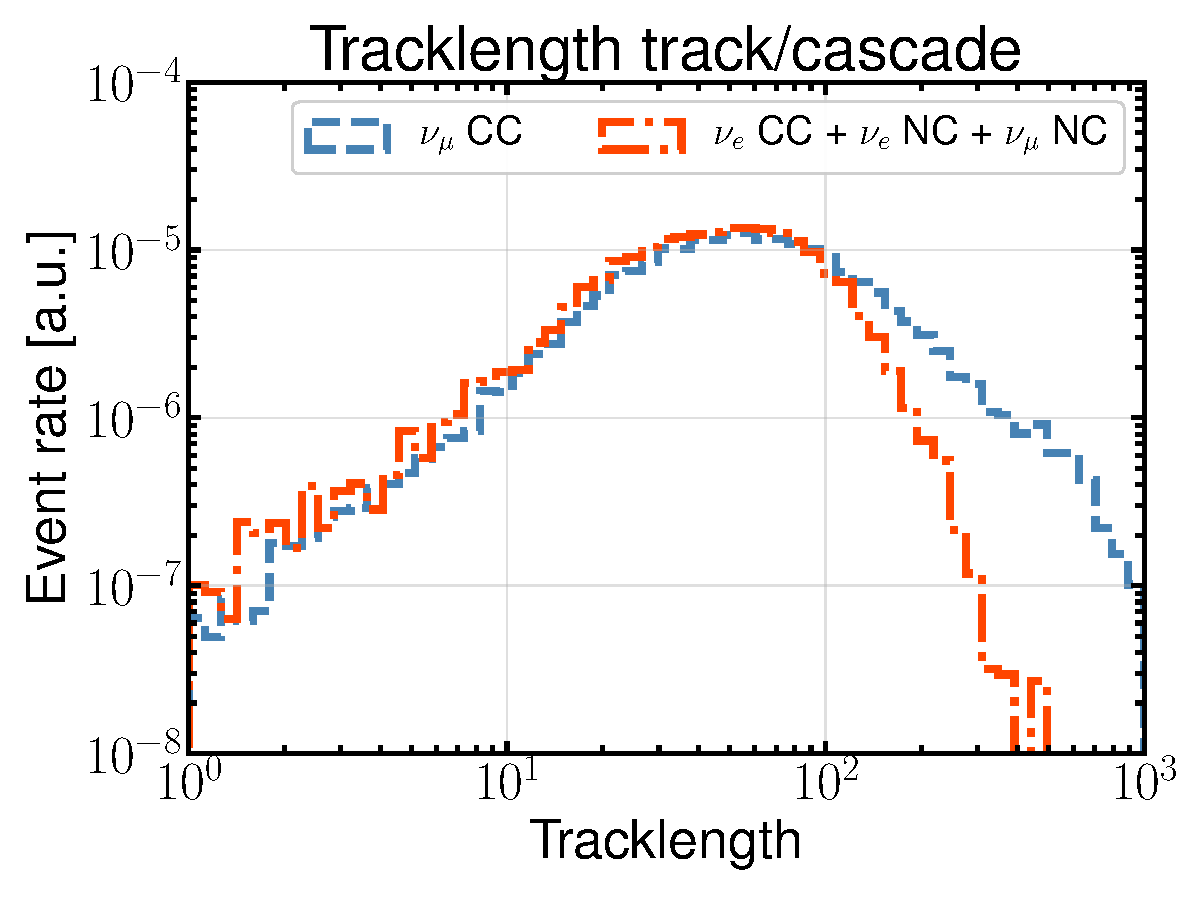
\includegraphics[width=0.49\linewidth]{figures/icecube/classification/variables/tracklength.pdf}
    \caption{Histogram of the reconstructed track length in simulation.}
    \label{fig:apx-pidvars-length}
\end{figure*}

\section{Three-flavor analysis}
\subsection{Seasonal Stability of Nuisance Parameter Fits}

\begin{figure}
    \centering
    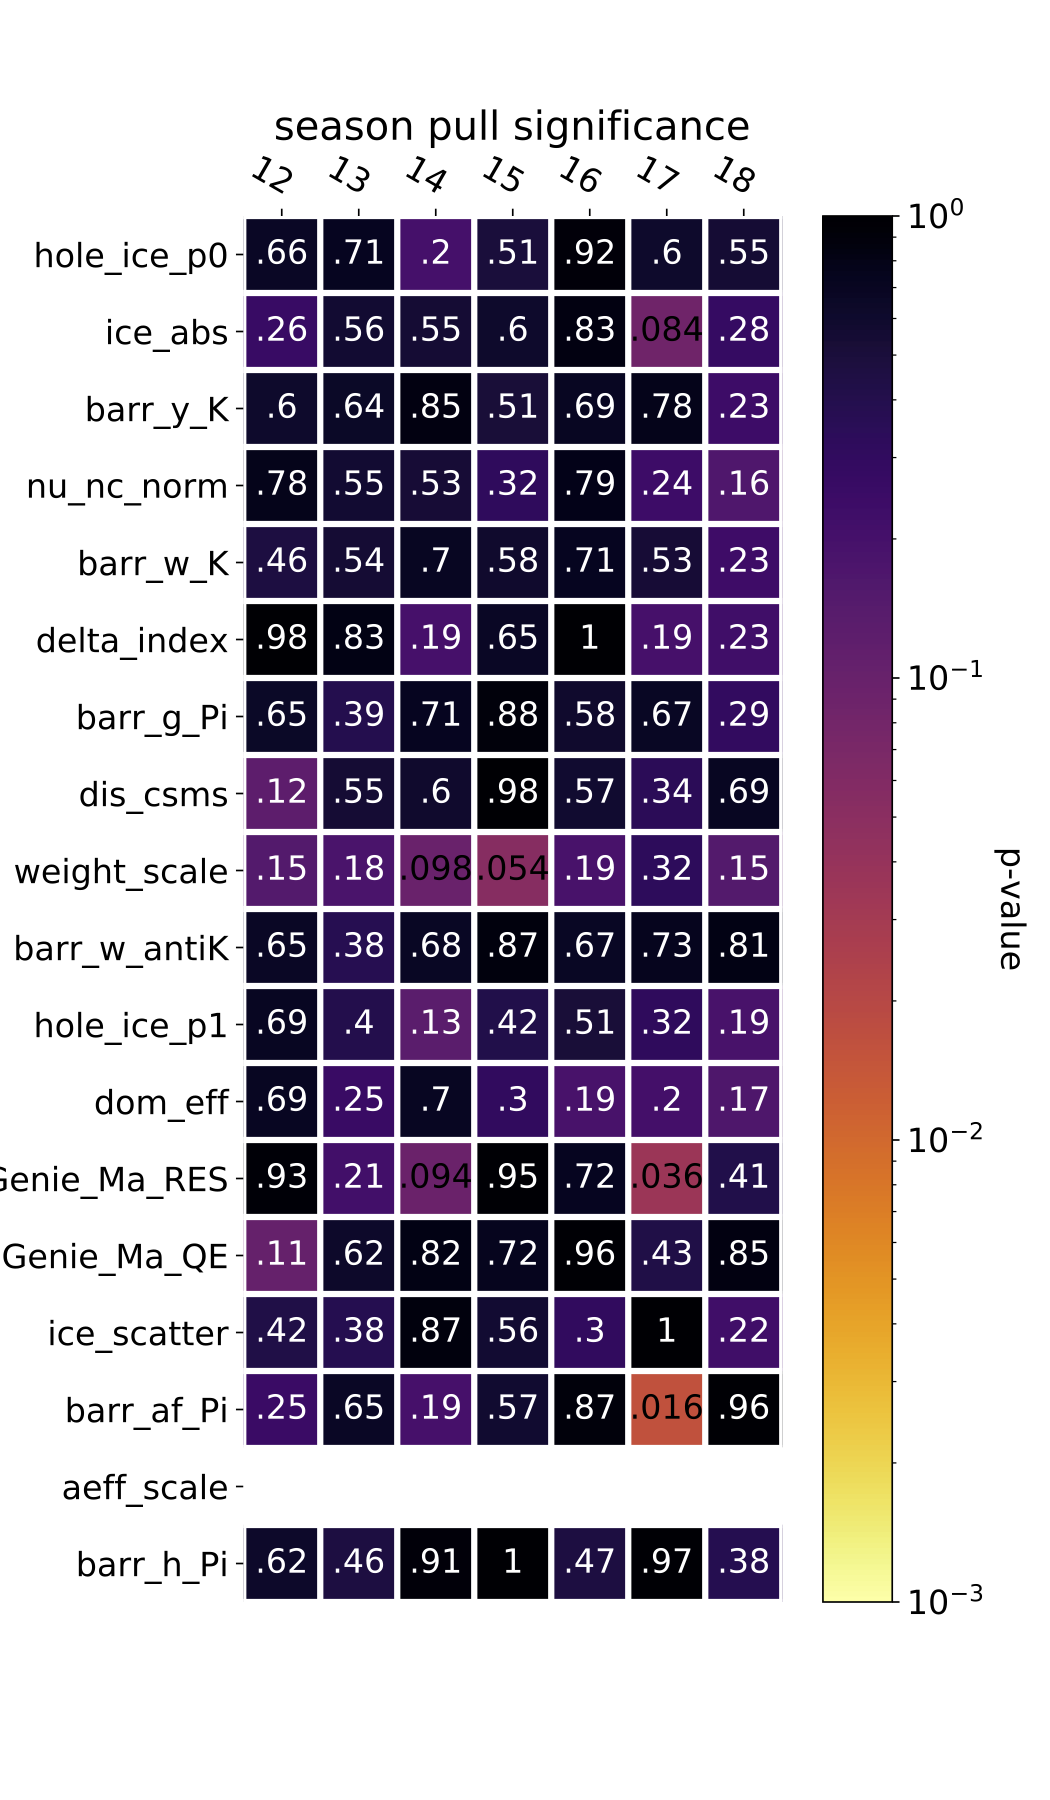
\includegraphics[width=0.8\textwidth]{figures/measurement/three_flavor/seasonal_stability/blind_ensemble_seasons_12-18_p-values.png}
    \caption{P-value of the blind ensemble test to ensure the compatibility of fit results of the three-flavor analysis between seasons. P-values are calculated using histograms of the fit results from an ensemble of pseudo-data where one year of live time is assumed for each trial. Season 2011 is excluded because its live time is smaller.\label{fig:pval-nuisance-parameter-ensemble}}
\end{figure}
